% !TeX spellcheck = en_US
\addscenariosection{1}{Cooperative scenario}{Malwick Proposal!}{\images/morale_high.png}

\begin{multicols*}{2}

\textbf{Author:} Invoceusse

\textbf{Source:} \href{https://discord.com/channels/740870068178649108/1230194988395270195}{Archon Studio Discord}

\textit{During your hunt in Emerald island someone help you... But now it's time to pay your debt!\\
The only way for paying this? Thief one of your new friend, but you know that friend keep what you need in the center of this town : so you can only fight it for claim it!\\
Fortunately your old friend can help you!
}

\subsection*{\MakeUppercase{Scenario Length}}

This scenario is played over 12 rounds.

\subsection*{\MakeUppercase{Player setup}}

\textbf{Player Count:} 1 -- 3

\textbf{Starting Resources:}\par
\resources{5}{2}{0}

\textbf{Starting Income:}\par
\resources{10}{0}{1}

\textbf{Starting Units:}
\begin{itemize}
  \item A Few \svgunit{silver} units of your choice.
\end{itemize}

\textbf{Town Buildings:} City Hall.

\textbf{Map tile Pool:} None.

\textbf{Additional Bonus:} None.

\subsection*{\MakeUppercase{Map Setup}}

Take the following Map tiles and arrange them as shown in the scenario map layout ($P$ stands for the number of players):

$\boldsymbol{2 P}$ \textbf{× Starting (I) Map tile}
$\boldsymbol{2 P}$ \textbf{× Far (II--III) Map tile}
$\boldsymbol{4 P}$ \textbf{× Far (IV--V) Map tile}
$\boldsymbol{1 P}$ \textbf{× Far (VI--VII) Map tile}
\begin{itemize}
    \item All the I tiles next to VI-VII tile are AI towns.
    \item Some tile can't be rotated.
\end{itemize}

\subsection*{\MakeUppercase{Victory Conditions}}

Flag all AI towns.

\subsection*{\MakeUppercase{Defeat Conditions}}

Lost battle again one AI.

\subsection*{\MakeUppercase{Timed Events}}

\textbf{\nth{6} Round:}
\begin{itemize}
  \item Choose one field with a black cube you can reach, then choose another player, he too gains the result of this field as if he visited it.
\end{itemize}
\textbf{end of \nth{12} Round:}
\begin{itemize}
    \item If you haven't reach your AI, immediately fight your AI but use turn 13 rule!
\end{itemize}

\subsection*{\MakeUppercase{Additional Rules}}
\begin{itemize}
    \item tile with yellow line in map cannot be rotated! If you draw one map with blocked field in center : your are lucky and can rotated as you want
    \item The first time during a round that one of your city buildings with "at the beginning" gives you a benefit, you must choose a different player to also gain this benefit at the beginning of this turn. You may also choose an another different player to gain this benefit instead of you.
    \item Whenever a player visits an Obelisk, that player rolls one treasure dice and one resource dice, chooses one of the dice and resolves its outcome dice.
    \item After defeating a level VII neutral army, instead of resolving the tile, draw 4 cards from the spell deck and/or artifact deck and one from deck deck or artifact deck or ability deck, add the first card of the spell/ability/artifact discard, you can add up to 2 of these 8 cards and gain 12 gold.
    \item When a player go into one Tile I their is not this faction, gain 1 MP.
    \item If you fight the AI for the first time (and not at end of Turn 12), you can keep your hand or draw again like at the start of a round. Also reset your crown.
    \item If you failed the last battle, you can have a second attempt, move your hero next to the AI town (and not in your town) then lose 2 experience level, then remove from the game the top 5 card of your deck.
    \item Additionally, no player can:
    \begin{itemize}
        \item Attack other Heroes.
        \item Capture a Mine or Settlement that is already Flagged.
    \end{itemize}
\end{itemize}

\vspace{2em}

\begin{center}
  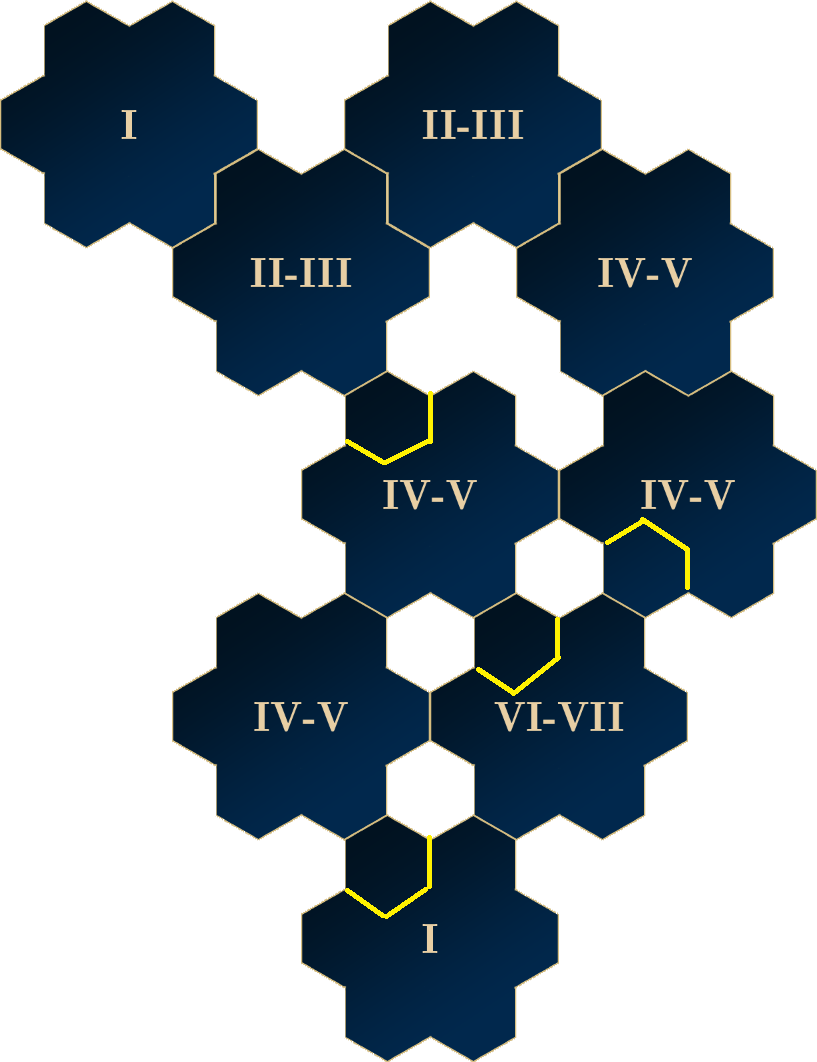
\includegraphics[width=0.35\paperwidth]{\_assets/maps/malwick_light_1.png}
  \captionof{figure}{1-PLAYER SCENARIO}
  \vspace{3em}
  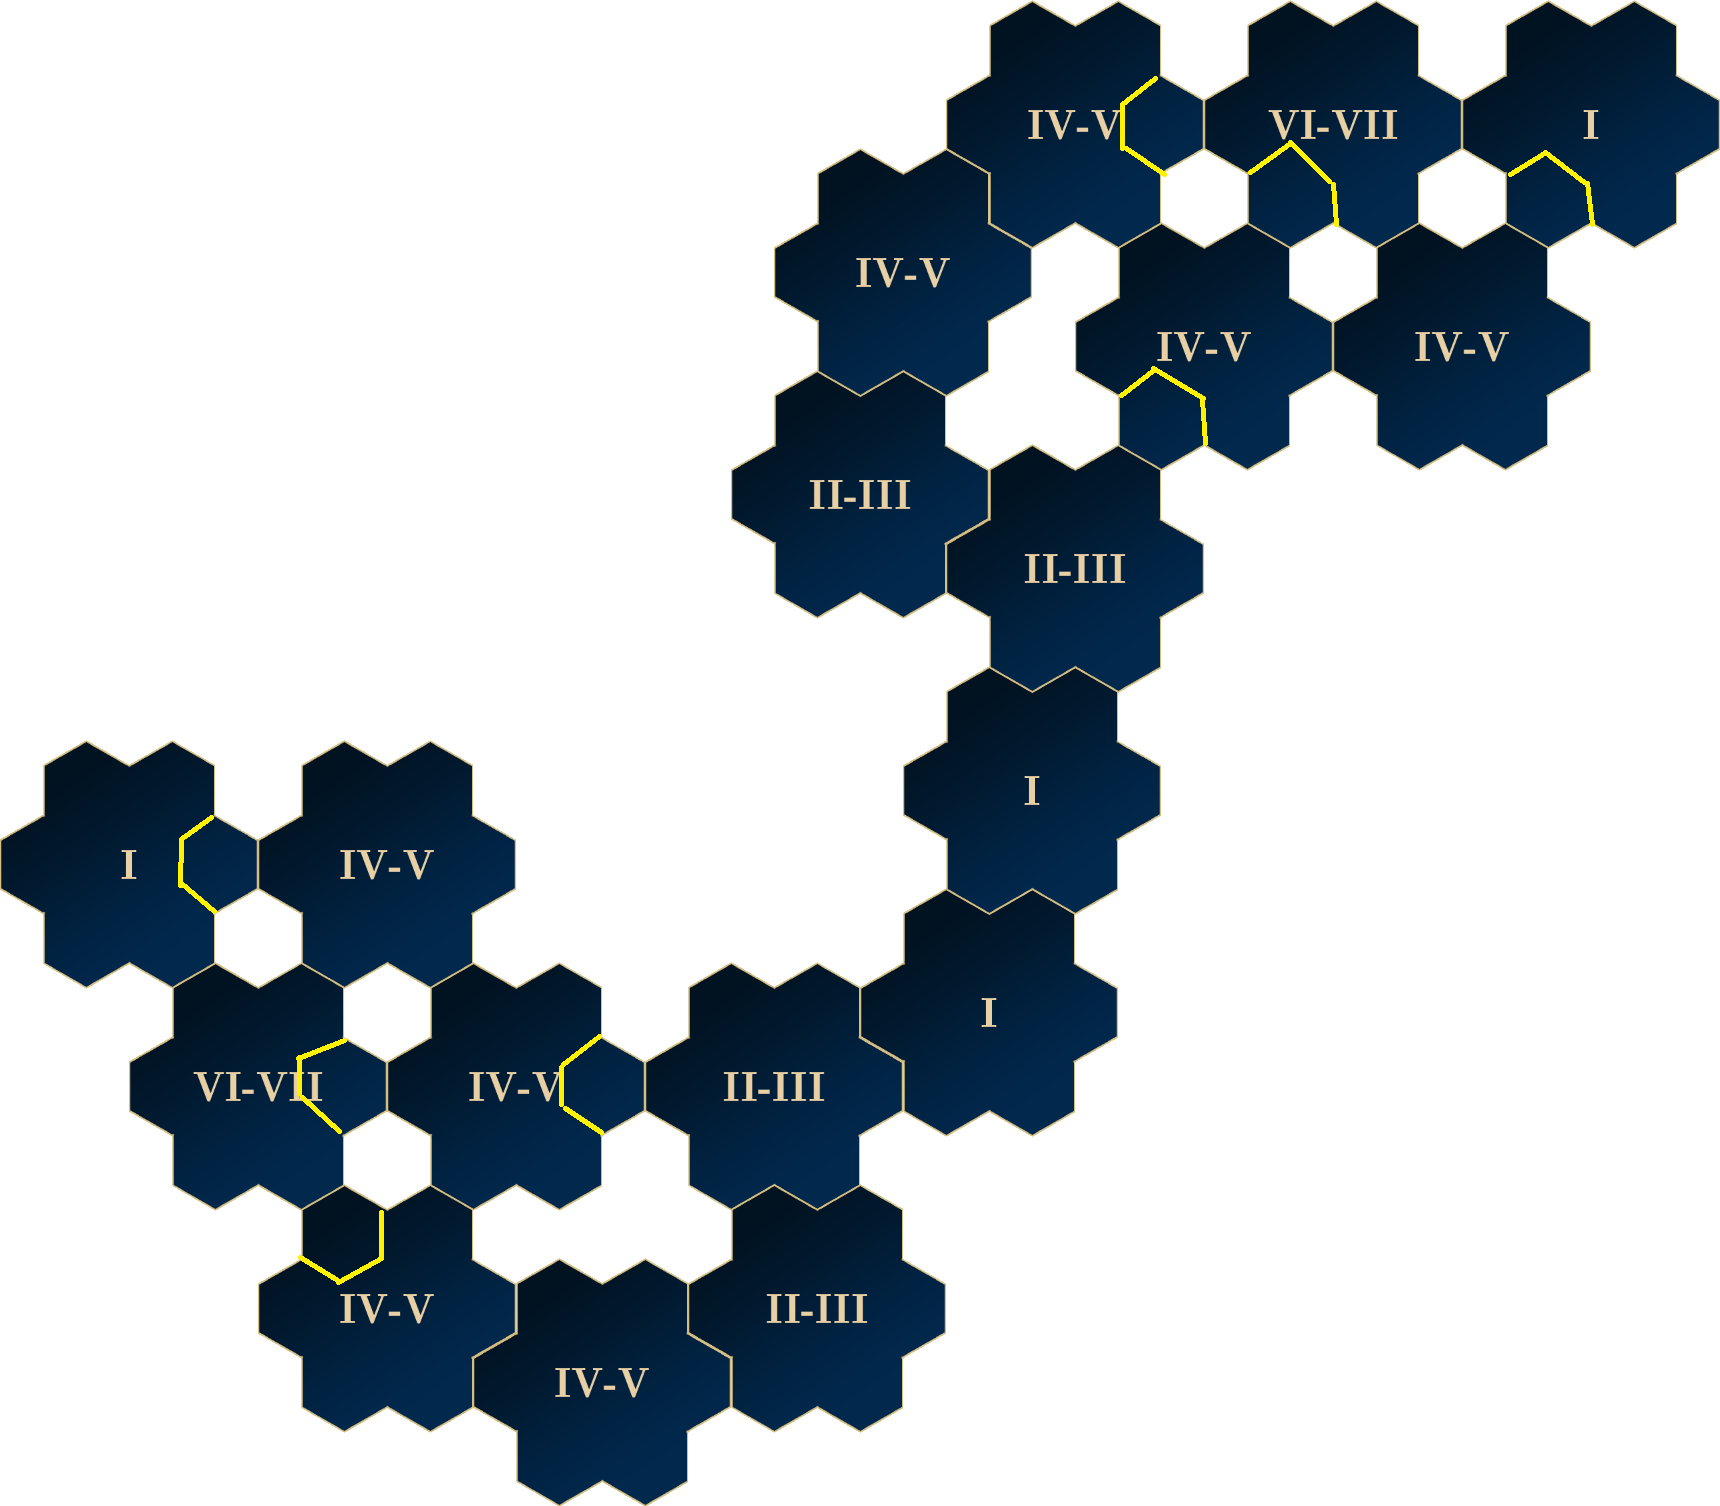
\includegraphics[width=0.45\paperwidth]{\_assets/maps/malwick_light_2.png}
  \captionof{figure}{2-PLAYER SCENARIO}
  \vspace{3em}
\end{center}

\end{multicols*}

\begin{center}
    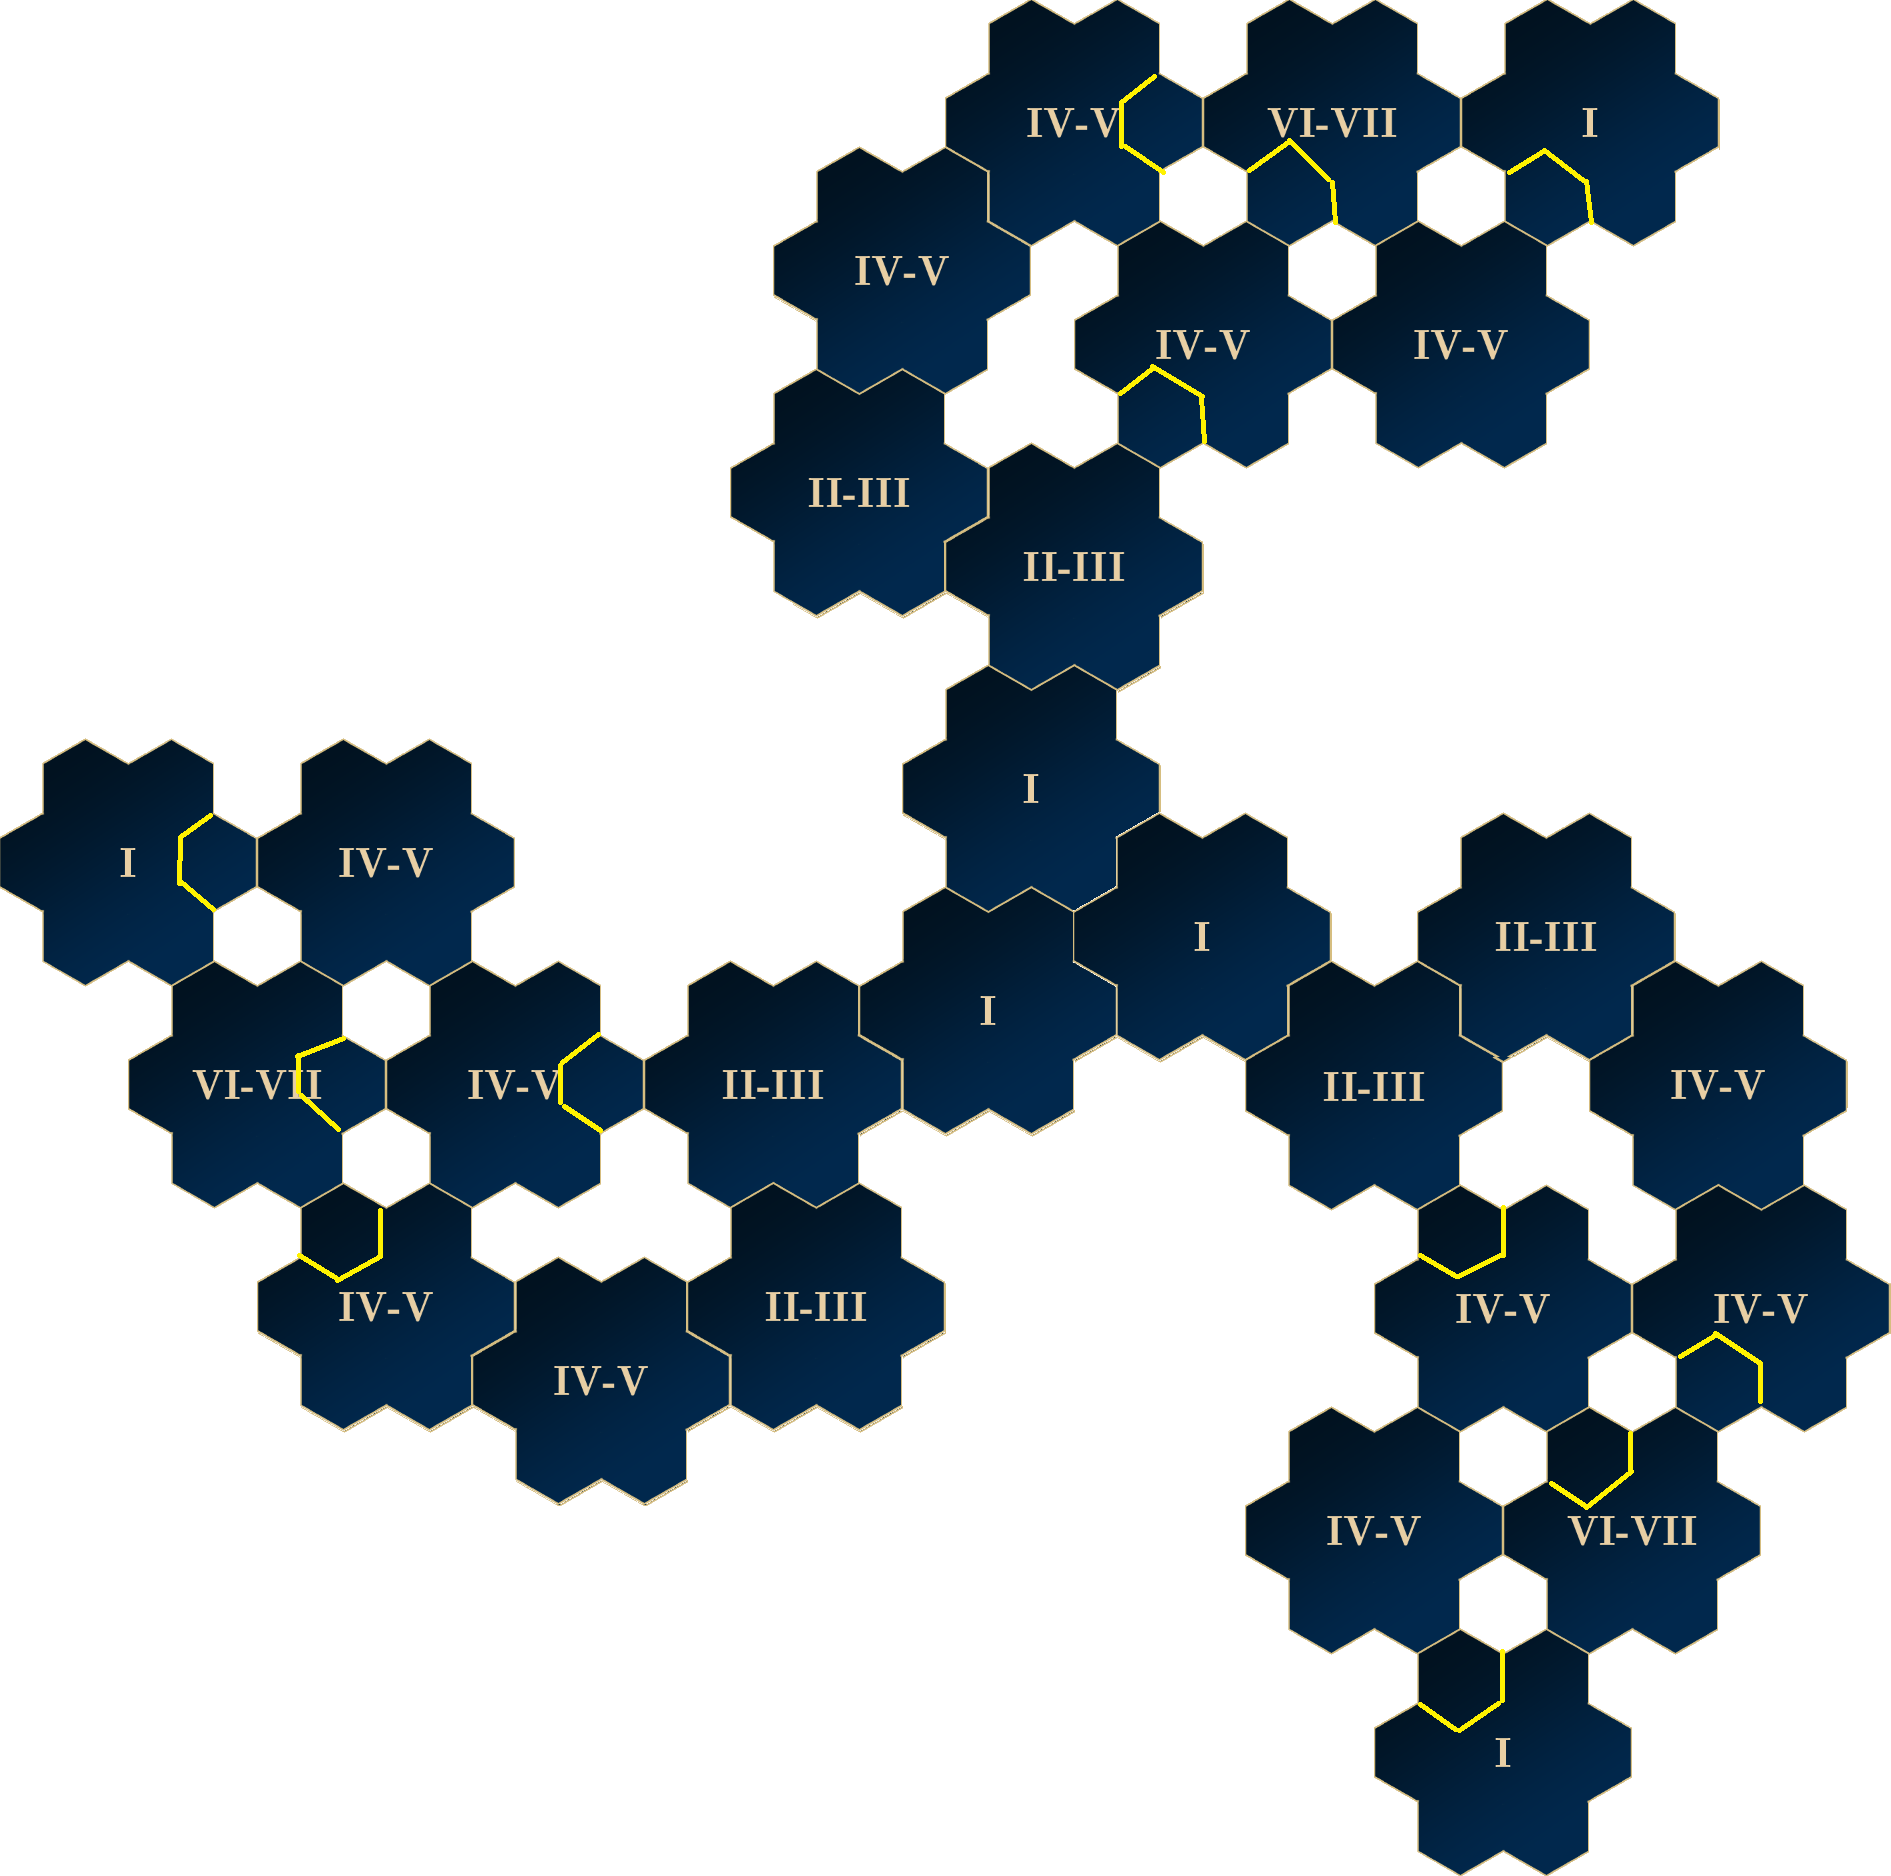
\includegraphics[width=0.8\paperwidth]{\_assets/maps/malwick_light_3.png}
    \captionof{figure}{3-PLAYER SCENARIO}
\end{center}
